\chapter{Ordinals}
\section{Counting for preschoolers}
In preschool, we were told to count as follows.
We defined a set of symbols $1$, $2$, $3$, $4$, \dots.
Then the teacher would hold up three apples and say:
\begin{quote}
	``One . . . two . . . three!  There are three apples.''
\end{quote}

\begin{center}
	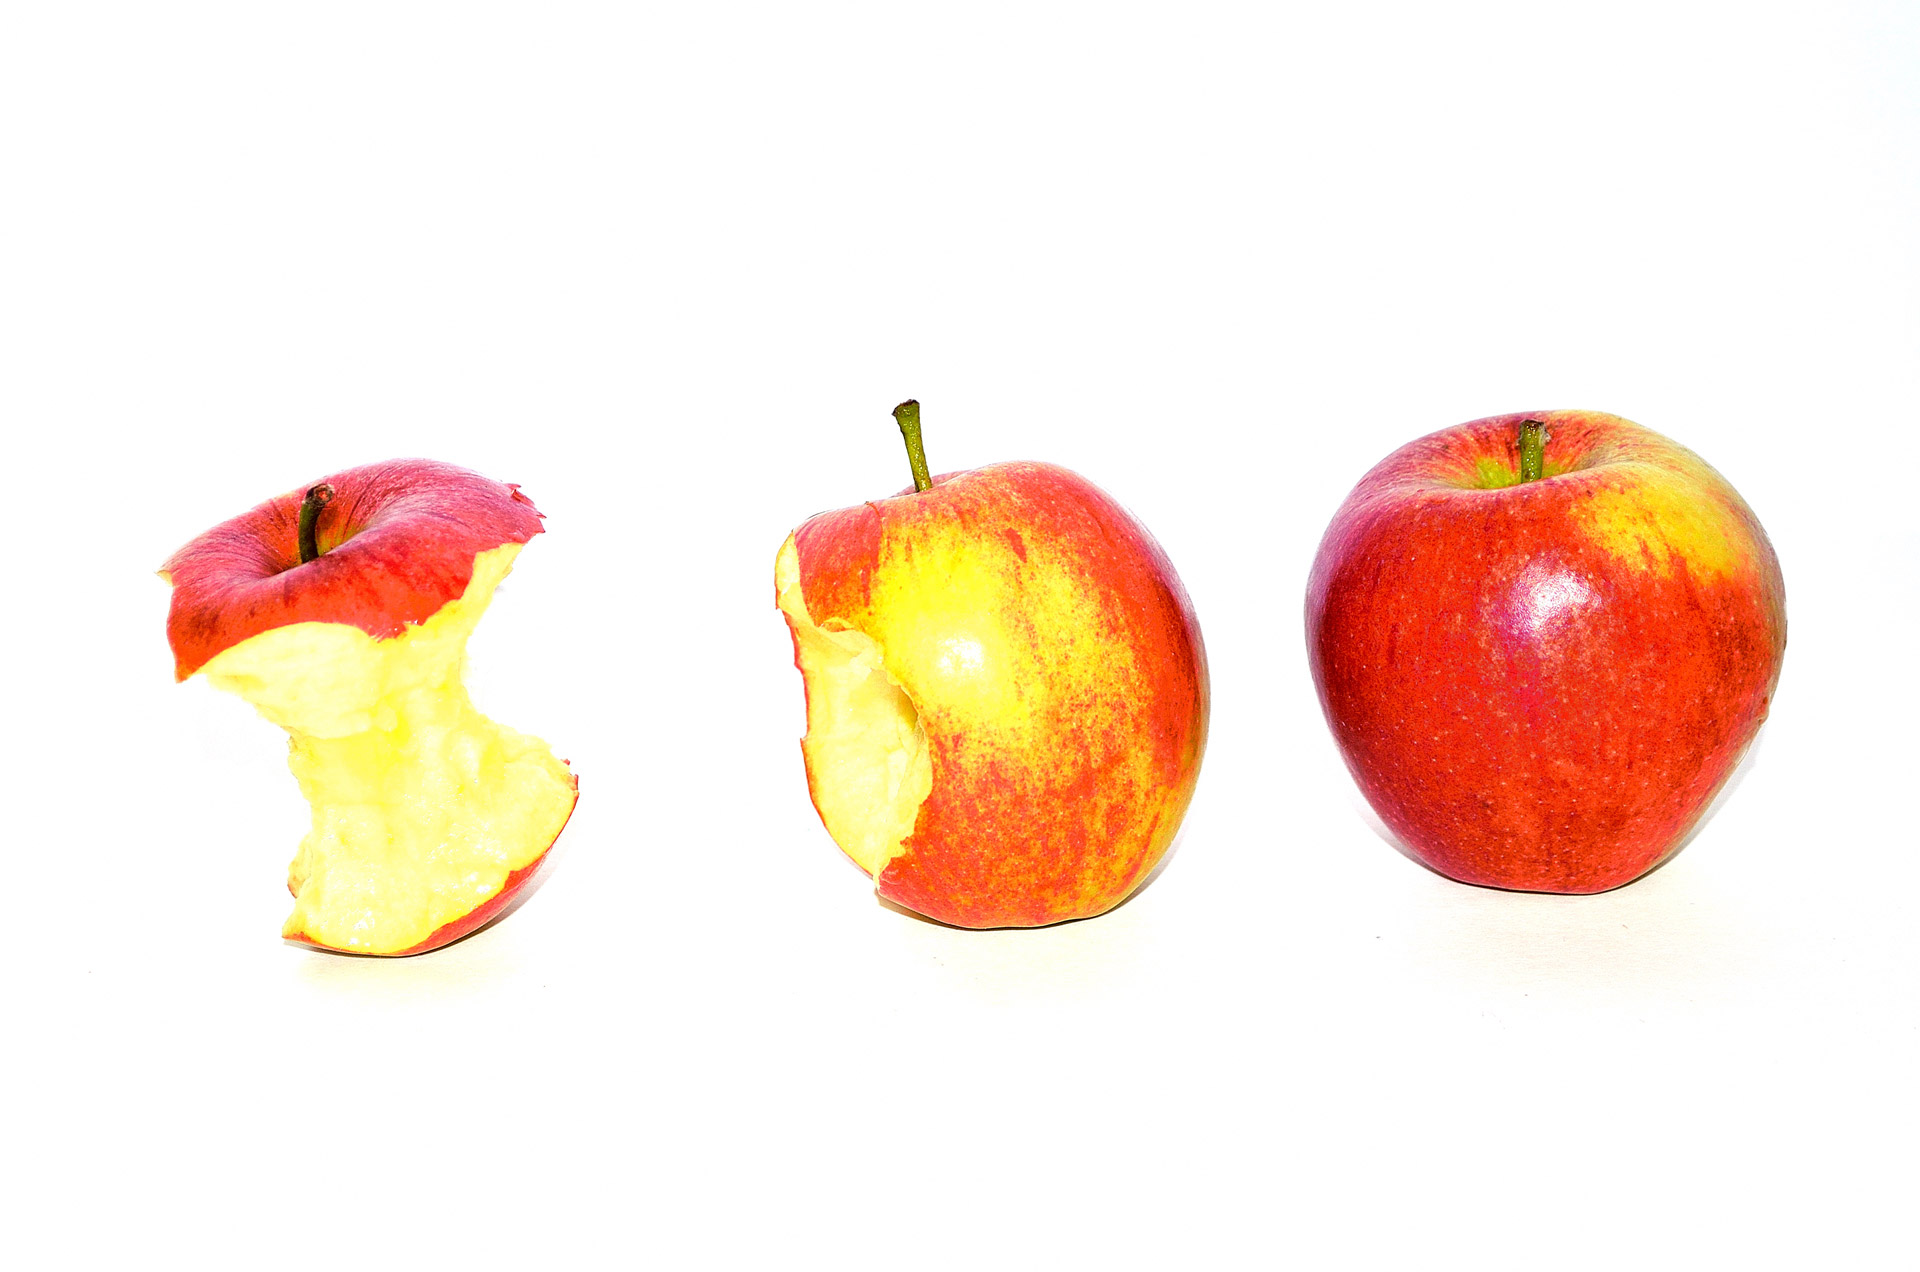
\includegraphics[height=5cm]{media/three-apples.jpg}
	\\ \scriptsize Image from \cite{img:apples}
\end{center}

The implicit definition is that the \emph{last} number said is the final answer.
This raises some obvious problems if we try to count infinite sets,
but even in the finite world,
this method of counting fails for the simplest set of all:
how many apples are in the following picture?

\begin{center}
	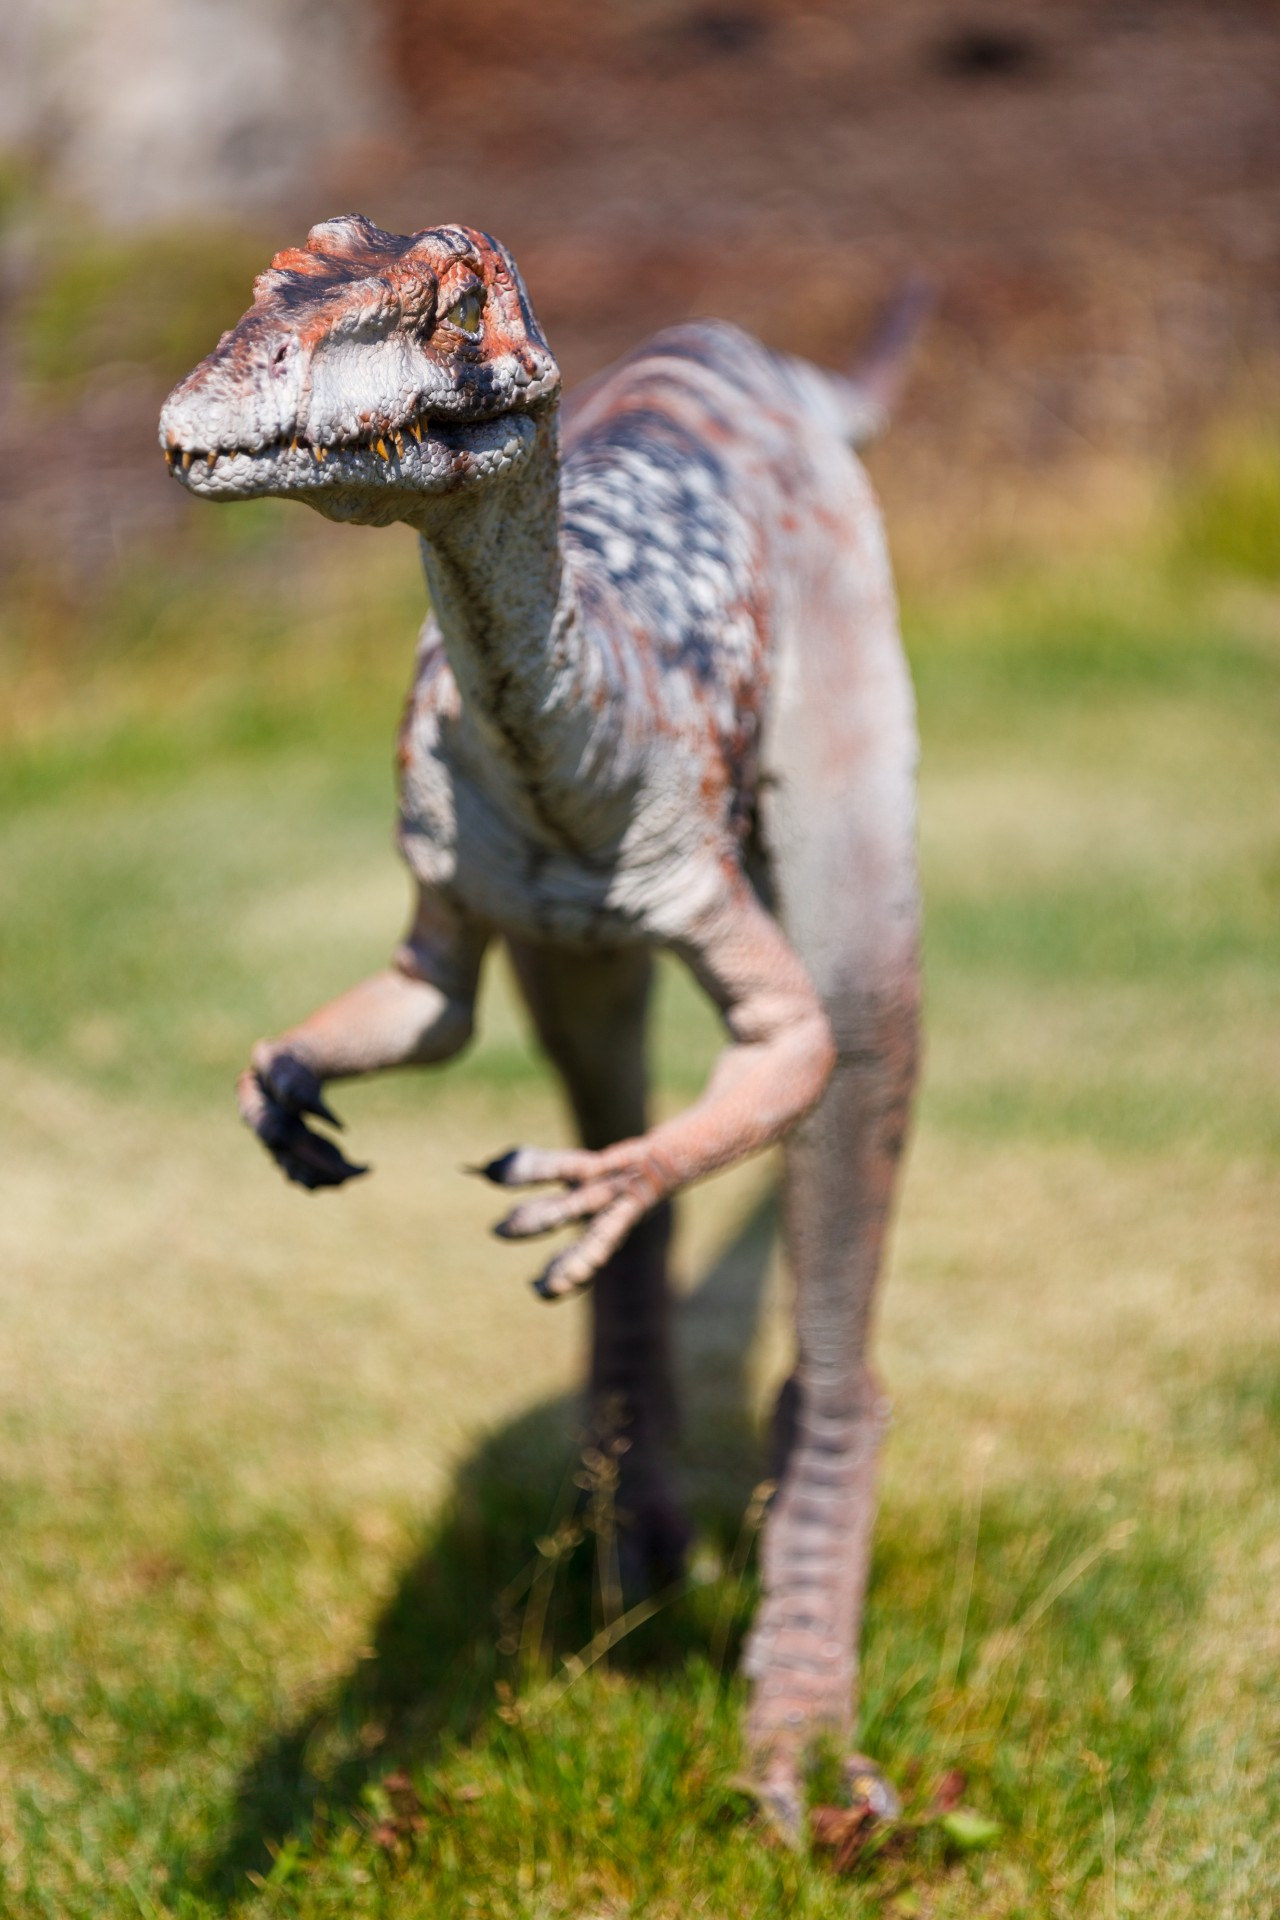
\includegraphics[height=7cm]{media/velociraptor.jpg}
	\\ \scriptsize Image from \cite{img:velociraptor}
\end{center}

Answer: $0$. There is nothing to say, and our method of counting has failed
for the simplest set of all: the empty set.

\section{Counting for set theorists}
\prototype{$\omega+1 = \{0,1,2,\dots,\omega\}$ might work.}
Rather than using the \emph{last} number listed, I propose instead
starting with a list of symbols $0$, $1$, $2$, \dots\ and making
the final answer the \emph{first} number which was \emph{not} said.
Thus to count three apples, we would say 
\begin{quote}
	``Zero . . . one . . . two!  There are three apples.''
\end{quote}
We will call these numbers \emph{ordinal numbers} (rigorous definition later).
In particular, we'll \emph{define} each ordinal to be the set of things we say:
\begin{align*}
	0 &= \varnothing \\
	1 &= \{0\} \\
	2 &= \{0,1\} \\
	3 &= \{0,1,2\} \\
	&\vdotswithin=
\end{align*}
In this way we can write out the natural numbers.
You can have some fun with this, by saying things like
\[
	4 \defeq
	\left\{ 
		\left\{  \right\},
		\left\{ \left\{  \right\} \right\},
		\left\{ \left\{  \right\}, \left\{ \left\{  \right\} \right\} \right\},
		\left\{ 
			\left\{  \right\},
			\left\{ \left\{  \right\} \right\},
			\left\{ \left\{  \right\}, \left\{ \left\{  \right\} \right\} \right\}
		\right\}
	\right\}
\]
In this way, we soon write down all the natural numbers.
The next ordinal, $\omega$,\footnote{
	That $\omega$ is actually a set is not obvious.
	The proof follows from the actual statement of $\Infinity$,
	which I've dutifully omitted.
	In fact, $\Infinity$ is equivalent to the existence of $\omega$.
} is defined as
\begin{align*}
	\omega &= \left\{ 0, 1, 2, \dots \right\} \\
	\intertext{Then comes}
	\omega+1 &= \left\{ 0, 1, 2, \dots, \omega \right\} \\
	\omega+2 &= \left\{ 0, 1, 2, \dots, \omega, \omega+1 \right\} \\
	\omega+3 &= \left\{ 0, 1, 2, \dots, \omega, \omega+1, \omega+2 \right\} \\
	&\vdotswithin= \\
	\intertext{And in this way we define $\omega+n$, and eventually reach}
	\omega \cdot 2 = \omega+\omega &= \left\{ 0, 1, 2 \dots, \omega, \omega+1, \omega+2, \dots \right\} \\
	\omega \cdot 2 + 1 &= \left\{ 0, 1, 2 \dots, \omega, \omega+1, \omega+2, \dots, \omega \cdot 2 \right\}.
\end{align*}
In this way we obtain
\begin{align*}
	0,\; & 1,\; 2,\; 3,\; \dots,\; \omega \\
	& \omega+1,\; \omega+2,\; \dots,\; \omega+\omega \\
	& \omega \cdot 2 +1,\; \omega \cdot 2 +2,\; \dots,\; \omega \cdot 3,\; \\
	& \vdots \\
	& \omega^2 + 1,\; \omega^2+2,\; \dots \\
	& \vdots \\
	& \omega^3,\; \dots,\; \omega^4,\; \dots,\; \omega^\omega \\
	& \vdots \\
	& \omega^{\omega^{\omega^{\dots}}} \\
\end{align*}

The first several ordinals can be illustrated in a nice spiral.
\begin{center}
	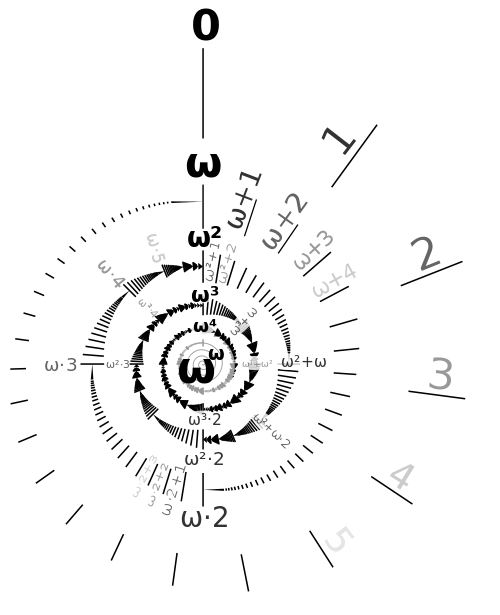
\includegraphics[scale=0.60]{media/500px-Omega-exp-omega-labeled.png}
\end{center}


\begin{remark}
	(Digression)
	The number $\omega^{\omega^{\omega^{\dots}}}$ has a name, $\eps_0$;
	it has the property that $\omega^{\eps_0} = \omega$.
	The reason for using ``$\eps$'' (which is usually used to denote small quantities)
	is that, despite how huge it may appear, it is actually a countable set.
	More on that later.
\end{remark}

\section{Definition of an ordinal}
Our informal description of ordinals gives us a chain
\[ 0 \in 1 \in 2 \in \dots \in \omega \in \omega+1 \in \dots. \]
To give the actual definition of an ordinal, I need to define two auxiliary terms first.
\begin{definition}
	A set $x$ is \vocab{transitive} if whenever $z \in y \in x$, we have $z \in x$ also.
\end{definition}
\begin{example}
	[$7$ is transitive]
	The set $7$ is transitive: for example, $2 \in 5 \in 7 \implies 2 \in 7$.
\end{example}
\begin{ques}
	Show that this is equivalent to: whenever $y \in x$, $y \subseteq x$.
\end{ques}
Moreover, recall the definition of ``well-ordering'': a strict linear order
with no infinite descending chains.
\begin{example}
	[$\in$ is a well-ordering on $\omega \cdot 3$]
	In $\omega \cdot 3$, we have an ordering
	\[ 0 \in 1 \in 2 \in \dots \in \omega \in \omega+1 \in \dots
		\in \omega \cdot 2 \in \omega \cdot 2 + 1 \in \dots. \]
	which has no infinite descending chains.
	Indeed, a typical descending chain might look like
	\[ \omega \cdot 2 + 6 \ni \omega \cdot 2 \ni
		\omega + 2015 \ni \omega+3 \ni \omega \ni 1000 \ni 256 \ni 42 \ni 7 \ni 0. \]
	Even though there are infinitely many elements, there is no way
	to make an infinite descending chain.
\end{example}
\begin{exercise}
	(Important)
	Convince yourself there are no infinite
	descending chains of ordinals at all,
	even without the $\Foundation$ axiom (which certainly implies this).
\end{exercise}

\begin{definition}
	An \vocab{ordinal} is a transitive set which is well-ordered by $\in$.
	The class of all ordinals is denoted $\On$.
\end{definition}

\begin{ques}
	Satisfy yourself that this definition works.
\end{ques}

We typically use Greek letters $\alpha$, $\beta$, etc.\ for ordinal numbers.
\begin{definition}
	We write
	\begin{itemize}
		\ii $\alpha < \beta$ to mean $\alpha \in \beta$,
		and $\alpha > \beta$ to mean $\alpha \ni \beta$.
		\ii $\alpha \le \beta$ to mean $\alpha \in \beta$ or $\alpha = \beta$,
		and $\alpha \ge \beta$ to mean $\alpha \ni \beta$ or $\alpha = \beta$,
	\end{itemize}
\end{definition}

\begin{theorem}[Ordinals are strictly ordered]
	Given any two ordinal numbers $\alpha$ and $\beta$,
	either $\alpha < \beta$, $\alpha = \beta$ or $\alpha > \beta$.
\end{theorem}
\begin{proof}
	Surprisingly annoying, thus omitted.
\end{proof}
\begin{theorem}[Ordinals represent all order types]
	Suppose $<$ is a well-ordering on a set $X$.
	Then there exists a unique ordinal $\alpha$
	such that there is a bijection $\alpha \to X$
	which is order preserving.
\end{theorem}
Thus ordinals represent the possible \emph{equivalence classes} of order types.
Any time you have a well-ordered set, it is isomorphic to a unique ordinal.

We now formalize the ``$+1$'' operation we were doing:
\begin{definition}
	Given an ordinal $\alpha$, we let $\alpha+1 = \alpha \cup \{\alpha\}$.
	An ordinal of the form $\alpha+1$ is called a \vocab{successor ordinal}.
\end{definition}
\begin{definition}
	If $\lambda$ is an ordinal which is neither zero nor a successor ordinal,
	then we say $\lambda$ is a \vocab{limit ordinal}.
\end{definition}
\begin{example}
	[Sucessor and limit ordinals]
	$7$, $\omega+3$, $\omega\cdot2+2015$ are successor ordinals,
	but $\omega$ and $\omega \cdot 2$ are limit ordinals.
\end{example}

\section{Ordinals are ``tall''}
First, we note that:
\begin{theorem}
	[There is no set of all ordinals]
	$\On$ is a proper class.
\end{theorem}
\begin{proof}
	Assume for contradiction not.
	Then $\On$ is well-ordered by $\in$ and transitive, so $\On$ is an ordinal,
	i.e.\ $\On \in \On$, which violates $\Foundation$.
\end{proof}
\begin{exercise}
	[Unimportant] Give a proof without $\Foundation$ by considering $\On+1$.
\end{exercise}

From this we deduce:
\begin{theorem}
	[Sets of ordinals are bounded]
	Let $A \subseteq \On$.
	Then there is some ordinal $\alpha$ such that $A \subseteq \alpha$
	(i.e.\ $A$ must be bounded).
\end{theorem}
\begin{proof}
	Otherwise, look at $\bigcup A$.
	It is a set.
	But if $A$ is unbounded it must equal $\On$,
	which is a contradiction.
\end{proof}
In light of this, every set of ordinals has a \vocab{supremum},
which is the least upper bound. We denote this by $\sup A$.

\begin{ques}
	Show that
	\begin{enumerate}[(a)]
		\ii $\sup (\alpha+1) = \alpha$ for any ordinal $\alpha$.
		\ii $\sup \lambda = \lambda$ for any limit ordinal $\lambda$.
	\end{enumerate}
\end{ques}

The pictorial ``tall'' will be explained in a few sections.

\section{Transfinite induction and recursion}
The fact that $\in$ has no infinite descending chains means that induction and recursion still work verbatim.
\begin{theorem}[Transfinite induction]
	Given a statement $P(-)$, suppose that
	\begin{itemize}
		\ii $P(0)$ is true, and
		\ii If $P(\alpha)$ is true for all $\alpha < \beta$, then $P(\beta)$ is true.
	\end{itemize}
	Then $P(\alpha)$ is true for every ordinal $\alpha$.
\end{theorem}
\begin{theorem}
	[Transfinite recursion]
	To define a sequence $x_\alpha$ for every ordinal $\alpha$,
	it suffices to
	\begin{itemize}
		\ii define $x_0$, then
		\ii for any $\beta$, define $x_\beta$ for any $\alpha < \beta$.
	\end{itemize}
\end{theorem}

The difference between this and normal induction lies in the \emph{limit ordinals}.
In real life, we might only do things like ``define $x_{n+1} = \dots$''.
But this is not enough to define $x_\alpha$ for all $\alpha$,
because we can't hit $\omega$ this way.
Similarly, the simple $+1$ doesn't let us hit the ordinal $2\omega$,
even if we already have $\omega+n$ for all $n$.
In other words, simply incrementing by $1$ cannot get us past limit stages,
but using transfinite induction to jump upwards lets us sidestep this issue.

So a transfinite induction or recursion is very often broken up into three cases.
In the induction phrasing, it looks like
\begin{itemize}
	\ii (Zero Case) First, resolve $P(0)$.
	\ii (Successor Case) Show that from $P(\alpha)$ we can get $P(\alpha+1)$.
	\ii (Limit Case) For $\lambda$ a limit ordinal,
	show that $P(\lambda)$ holds given $P(\alpha)$ for all $\alpha < \lambda$,
	where $\lambda$ is a limit ordinal.
\end{itemize}
Similarly, transfinite recursion often is split into cases too.
\begin{itemize}
	\ii (Zero Case) First, define $x_0$.
	\ii (Successor Case) Define $x_{\alpha+1}$ from $x_\alpha$.
	\ii (Limit Case) Define $x_\lambda$ from $x_\alpha$ for all $\alpha < \lambda$,
	where $\lambda$ is a limit ordinal.
\end{itemize}
In both situations, finite induction only does the first two cases,
but if we're able to do the third case we can climb above the barrier $\omega$.

\section{Ordinal arithmetic}
\prototype{$1+\omega=\omega \neq \omega+1$.}
To give an example of transfinite recursion, let's define addition of ordinals.
Recall that we defined $\alpha+1 = \alpha \cup \{\alpha\}$.
By transfinite recursion, let
\begin{align*}
	\alpha + 0 &= \alpha \\
	\alpha + (\beta + 1) &= (\alpha + \beta) + 1 \\
	\alpha + \lambda &= \bigcup_{\beta < \lambda} (\alpha + \beta).
\end{align*}
Here $\lambda \neq 0$.

We can also do this explicitly:
The picture is to just line up $\alpha$ after $\beta$.
That is, we can consider the set
\[
	X = 
	\left( \left\{ 0 \right\} \times \alpha \right)
	\cup
	\left( \left\{ 1 \right\} \times \beta \right)
\]
(i.e.\ we tag each element of $\alpha$ with a $0$, and
each element of $\beta$ with a $1$).
We then impose a well-ordering on $X$ by a lexicographic ordering $\llex$
(sort by first component, then by second).
This well-ordering is isomorphic to a unique ordinal, 
\begin{example}
	[$2+3=5$]
	Under the explicit construction for $\alpha = 2$ and $\beta = 3$, we get the set
	\[
		X = \left\{ (0,0) < (0,1) < (1,0) < (1,1) < (1,2) \right\}
	\]
	which is isomorphic to $5$.
\end{example}

\begin{example}[Ordinal arithmetic is not commutative]
	Note that $1 + \omega = \omega$!
	Indeed, under the transfinite definition, we have
	\[ 1 + \omega = \cup_n (1+n) = 2 \cup 3 \cup 4 \cup \dots = \omega. \]
	With the explicit construction, we have
	\[ X = \left\{ (0,0) < (1,0) < (1,1) < (1,2) < \dots \right\} \]
	which is isomorphic to $\omega$.
\end{example}
\begin{exercise}
	Show that $n+\omega = \omega$ for any $n \in \omega$.
\end{exercise}

\begin{remark}
	Ordinal addition is not commutative.
	However, from the explicit construction
	we can see that it is at least associative.
\end{remark}

Similarly, we can define multiplication in two ways.
By transfinite induction:
\begin{align*}
	\alpha \cdot 0 &= 0 \\
	\alpha \cdot (\beta + 1) &= (\alpha \cdot \beta) + \alpha \\
	\alpha \cdot \lambda &= \bigcup_{\beta < \lambda} \alpha \cdot \beta.
\end{align*}
We can also do an explicit construction: $\alpha \cdot \beta$
is the order type of
\[ \llex \text{ applied to } \beta \times \alpha. \]
\begin{example}[Ordinal multiplication is not commutative]
	We have $\omega \cdot 2 = \omega + \omega$,
	but $2 \cdot \omega = \omega$.
\end{example}
\begin{exercise}
	Prove this.
\end{exercise}
\begin{exercise}
	Verify that ordinal multiplication
	(like addition) is associative but not commutative.
	(Look at $\gamma \times \beta \times \alpha$.)
\end{exercise}

Exponentiation can also be so defined, though the explicit construction is less natural.
\begin{align*}
	\alpha^0 &= 1 \\
	\alpha^{\beta+1} &= \alpha^{\beta} \cdot \alpha \\
	\alpha^{\lambda} &= \bigcup_{\beta < \lambda} \alpha^\beta.
\end{align*}
\begin{exercise}
	Verify that $2^\omega = \omega$.
\end{exercise}


\section{The hierarchy of sets}
We now define the \vocab{von Neumann Hierarchy} by transfinite recursion.
\begin{definition}
	By transfinite recursion, we set
	\begin{align*}
		V_0 &= \varnothing \\
		V_{\alpha + 1} &= \PP(V_\alpha) \\
		V_\lambda &= \bigcup_{\alpha<\lambda} V_\alpha
	\end{align*}
\end{definition}
By transfinite induction, we see $V_\alpha$ is transitive
and that $V_\alpha \subseteq V_\beta$ for all $\alpha < \beta$.

\begin{example}[$V_\alpha$ for $\alpha \le 3$]
	The first few levels of the hierarchy are:
	\begin{align*}
		V_0 &= \varnothing \\
		V_1 &= \left\{ 0 \right\} \\
		V_2 &=  \left\{ 0, 1 \right\} \\
		V_3 &= \left\{ 0, 1, 2, \left\{ 1 \right\} \right\}.
	\end{align*}
	Notice that for each $n$, $V_n$ consists of only finite sets,
	and each $n$ appears in $V_{n+1}$ for the first time.
	Observe that
	\[ V_\omega = \bigcup_{n \in \omega} V_n \]
	consists only of finite sets; thus $\omega$ appears for the first time
	in $V_{\omega+1}$.
\end{example}
\begin{ques}
	How many sets are in $V_5$?
\end{ques}

\begin{definition}
	The \vocab{rank} of a set $y$, denoted $\rank(y)$,
	is the smallest ordinal $\alpha$ such that $y \in V_{\alpha+1}$.
\end{definition}
\begin{example}
	$\rank(2) = 2$, and actually $\rank(\alpha)=\alpha$
	for any ordinal $\alpha$ (problem later).
	This is the reason for the extra ``$+1$''.
\end{example}
\begin{ques}
	Show that $\rank(y)$ is the smallest ordinal $\alpha$
	such that $y \subseteq V_\alpha$.
\end{ques}

It's not yet clear that the rank of a set actually exists, so we prove:
\begin{theorem}[The von Neumann hierachy is complete]
	The class $V$ is equal to $\bigcup_{\alpha \in \On} V_\alpha$.
	In other words, every set appears in some $V_\alpha$.
\end{theorem}
\begin{proof}
	Assume for contradiction this is false.
	The key is that because $\in$ satisfies $\Foundation$,
	we can take a $\in$-minimal counterexample $x$.
	Thus $\rank(y)$ is defined for every $y \in x$,
	and we can consider (by $\Replacement$) the set
	\[ \left\{ \rank(y) \mid y \in x \right\}. \]
	Since it is a set of ordinals, it is bounded.
	So there is some large ordinal $\alpha$ such that $y \in V_\alpha$
	for all $y \in x$, i.e.\ $x \subseteq V_\alpha$,
	so $x \in V_{\alpha+1}$.
\end{proof}

This leads us to a picture of the universe $V$:
\begin{center}
	\begin{asy}
		size(11cm);
		pair A = (12,30);
		pair B = -conj(A);
		pair M = midpoint(A--B);
		pair O = origin;
		MP("V", A, dir(10));
		draw(A--O--B);

		fill(A--O--B--cycle, opacity(0.3)+palecyan);

		MP("V_0 = \varnothing", origin, dir(-20));
		MP("V_1 = \{\varnothing\}", 0.05*A, dir(0));
		MP("V_2 = \{\varnothing, \{\varnothing\} \}", 0.10*A, dir(0));

		draw(MP("V_n", 0.3*A, dir(0))--0.3*B);
		draw(MP("V_{n+1} = \mathcal P(V_n)", 0.35*A, dir(0))--0.35*B);
		Drawing("n", 0.35*M, dir(45));

		draw(MP("V_\omega = \bigcup V_n", 0.5*A, dir(0))--0.5*B);
		draw(MP("V_{\omega+1} = \mathcal P(V_{\omega})", 0.55*A, dir(0))--0.55*B);
		Drawing("\omega", 0.55*M, dir(45));
		draw(MP("V_{\omega+2} = \mathcal P(V_{\omega+1})", 0.6*A, dir(0))--0.6*B);
		Drawing("\omega+1", 0.6*M, dir(45));

		draw(MP("V_{\omega+\omega}", 0.8*A, dir(0))--0.8*B);

		draw(origin--M);
		MP("\mathrm{On}", M, dir(90));

	\end{asy}
\end{center}

We can imagine the universe $V$ as a triangle,
built in several stages or layers,
$V_0 \subsetneq V_1 \subsetneq V_2 \subsetneq \dots$.
This universe doesn't have a top: but each of the $V_i$ do.
However, the universe has a very clear bottom.
Each stage is substantially wider than the previous one.

In the center of this universe are the ordinals:
for every successor $V_\alpha$, exactly one new ordinal appears, namely $\alpha$.
Thus we can picture the class of ordinals as a thin line
that stretches the entire height of the universe.
A set has rank $\alpha$ if it appears at the same stage that $\alpha$ does.


All of number theory, the study of the integers, lives inside $V_\omega$.
Real analysis, the study of real numbers, lives inside $V_{\omega+1}$, since a real number
can be encoded as a subset of $\NN$ (by binary expansion).
Functional analysis lives one step past that, $V_{\omega+2}$.
For all intents and purposes, most mathematics does not go beyond $V_{\omega+\omega}$.
This pales in comparison to the true magnitude of the whole universe.

\section\problemhead
\begin{problem}
	Prove that $\rank(\alpha) = \alpha$ for any $\alpha$
	by transfinite induction.
\end{problem}

\begin{problem}
	[Online Math Open]
	Count the number of transitive sets in $V_5$.
\end{problem}

\begin{problem}
	[Goodstein]
	Let $a_2$ be any positive integer.
	We define the infinite sequence $a_2$, $a_3$, \dots recursively as follows.
	If $a_{n} = 0$, then $a_{n+1} = 0$.
	Otherwise, we write $a_n$ in base $n$,
	then write all exponents in base $n$, and so on until all
	numbers in the expression are at most $n$.
	Then we replace all instances of $n$ by $n+1$
	(including the exponents!), subtract $1$,
	and set the result to $a_{n+1}$.
	For example, if $a_2 = 11$ we have
		\begin{align*}
			a_2 &= 2^{3} + 2 + 1 = 2^{2+1} + 2 + 1 \\
			a_3 &= 3^{3+1}+3+1-1 = 3^{3+1} + 3\\
			a_4 &= 4^{4+1} + 4 - 1 = 4^{4+1} + 3 \\
			a_5 &= 5^{5+1} + 3 - 1 = 5^{5+1} + 2
		\end{align*}
	and so on. Prove that $a_N = 0$ for some integer $N > 2$.
\end{problem}
